%----------------------------------------------------------------------------------------
%	EXAMPLE AND DOCUMENTATION OF THE KAOBOOK CLASS
%----------------------------------------------------------------------------------------

\documentclass[
	a4paper, % Page size
	fontsize=10pt, % Base font size
    twoside=true, % Use different layouts for even and odd pages (in particular, if twoside=true, the margin column will be always on the outside)
	%open=any, % If twoside=true, uncomment this to force new chapters to start on any page, not only on right (odd) pages
	%chapterentrydots=true, % Uncomment to output dots from the chapter name to the page number in the table of contents
	numbers=noenddot, % Comment to output dots after chapter numbers; the most common values for this option are: enddot, noenddot and auto (see the KOMAScript documentation for an in-depth explanation)
]{kaobook}

%----------------------------------------------------------------------------------------
%	PACKAGES AND OTHER DOCUMENT CONFIGURATIONS
%----------------------------------------------------------------------------------------

% Choose the language
\ifxetexorluatex
	\usepackage{polyglossia}
	\setmainlanguage[variant=mexican]{spanish}
\else
	\usepackage[spanish,mexico]{babel} % Load characters and hyphenation
\fi
\usepackage[autostyle]{csquotes}	% English quotes

% Load packages for testing
%\usepackage{blindtext}
%\usepackage{showframe} % Uncomment to show boxes around the text area, margin, header and footer
%\usepackage{showlabels} % Uncomment to output the content of \label commands to the document where they are used

% Load the bibliography package
\usepackage{styles/kaobiblio}
\addbibresource{bib.bib} % Bibliography file

% Load mathematical packages for theorems and related environments. NOTE: choose only one between 'mdftheorems' and 'plaintheorems'.
\usepackage{styles/mdftheorems}
%\usepackage{styles/plaintheorems}

% Load the package for hyperreferences
\usepackage{styles/kaorefs}

% Sistema Internacional de Unidades
\usepackage{siunitx}
\DeclareSIUnit\Molar{\textsc{m}} % Unidades de molaridad

% Para reacciones químicas
\usepackage[version=4]{mhchem}
 
\graphicspath{imgs/} % Paths in which to look for images

\makeindex[columns=3, title=Alphabetical Index, intoc] % Make LaTeX produce the files required to compile the index

\makeglossaries % Make LaTeX produce the files required to compile the glossary
\input{glossary.tex} % Include the glossary definitions

\makenomenclature % Make LaTeX produce the files required to compile the nomenclature

% Reset sidenote counter at chapters
%\counterwithin*{sidenote}{chapter}

%----------------------------------------------------------------------------------------

\begin{document}

%----------------------------------------------------------------------------------------
%	BOOK INFORMATION
%----------------------------------------------------------------------------------------

%\titlehead{Lolo}
%\subject{Lola}

\title[Efecto del pH en el daño por radiación]{Efecto del pH en la condición de cristalización sobre el daño por radiación en cristales de proteína}
%\subtitle{Customise this page according to your needs}

\author[FMP]{Francisco Murphy Pérez}

\date{\today}

%\publishers{An Awesome Publisher}

%----------------------------------------------------------------------------------------

\frontmatter % Denotes the start of the pre-document content, uses roman numerals

%----------------------------------------------------------------------------------------
%	OPENING PAGE
%----------------------------------------------------------------------------------------

%\makeatletter
%\extratitle{
%	% In the title page, the title is vspaced by 9.5\baselineskip
%	\vspace*{9\baselineskip}
%	\vspace*{\parskip}
%	\begin{center}
%		% In the title page, \huge is set after the komafont for title
%		\usekomafont{title}\huge\@title
%	\end{center}
%}
%\makeatother

%----------------------------------------------------------------------------------------
%	COPYRIGHT PAGE
%----------------------------------------------------------------------------------------

\makeatletter
%\uppertitleback{\@titlehead} % Header

\lowertitleback{
%	\textbf{Disclaimer}\\
%	You can edit this page to suit your needs. For instance, here we have a no copyright statement, a colophon and some other information. This page is based on the corresponding page of Ken Arroyo Ohori's thesis, with minimal changes.
%	
	\medskip
%	
%	\textbf{No copyright}\\
%	\cczero\ This book is released into the public domain using the CC0 code. To the extent possible under law, I waive all copyright and related or neighbouring rights to this work.
%	
%	To view a copy of the CC0 code, visit: \\\url{http://creativecommons.org/publicdomain/zero/1.0/}
%	
	\medskip
	
	\textbf{Colofón} \\
	Este documento se compuso con la ayuda de \href{https://sourceforge.net/projects/koma-script/}{\KOMAScript} and \href{https://www.latex-project.org/}{\LaTeX} usando la plantilla \href{https://github.com/fmarotta/kaobook/}{kaobook}.
	
%	The source code of this book is available at:\\\url{https://github.com/fmarotta/kaobook}
	
%	(You are welcome to contribute!)
	
	\medskip
	
%	\textbf{Publisher} \\
%	First printed in May 2019 by \@publishers
}
\makeatother

%----------------------------------------------------------------------------------------
%	DEDICATION
%----------------------------------------------------------------------------------------

\dedication{
	A Lucía, por supuesto.\\
	\flushright -- Con todo mi amor.
}

%----------------------------------------------------------------------------------------
%	OUTPUT TITLE PAGE AND PREVIOUS
%----------------------------------------------------------------------------------------

% Note that \maketitle outputs the pages before here

% If twoside=false, \uppertitleback and \lowertitleback are not printed
% To overcome this issue, we set twoside=semi just before printing the title pages, and set it back to false just after the title pages
\KOMAoptions{twoside=semi}
\maketitle
\KOMAoptions{twoside=false}

%----------------------------------------------------------------------------------------
%	PREFACE
%----------------------------------------------------------------------------------------

\chapter*{Resumen}
Aquí va el resumen, normalmente esto se escribe al final de la tesis.

\index{preface}

%----------------------------------------------------------------------------------------
%	TABLE OF CONTENTS & LIST OF FIGURES/TABLES
%----------------------------------------------------------------------------------------

\begingroup % Local scope for the following commands

% Define the style for the TOC, LOF, and LOT
%\setstretch{1} % Uncomment to modify line spacing in the ToC
%\hypersetup{linkcolor=blue} % Uncomment to set the colour of links in the ToC
\setlength{\textheight}{230\hscale} % Manually adjust the height of the ToC pages

% Turn on compatibility mode for the etoc package
\etocstandarddisplaystyle % "toc display" as if etoc was not loaded
\etocstandardlines % "toc lines as if etoc was not loaded

\tableofcontents % Output the table of contents

\listoffigures % Output the list of figures

% Comment both of the following lines to have the LOF and the LOT on different pages
%\let\cleardoublepage\bigskip
%\let\clearpage\bigskip

\listoftables % Output the list of tables



\newacronym{api}{API}{Application Programming Interface }
\newacronym{pdb}{PDB}{Protein Data Bank}
\newacronym{crx}{CRX}{Cristalografía de rayos X}
\newacronym{ccd}{CCD}{Charge-coupled device}
\newacronym{xfel}{XFEL}{X-ray Free Electron Laser}
\newacronym{iupac}{IUPAC}{International Union of Pure and Applied Chemistry}
\setglossarystyle{listgroup} % Set the style of the glossary (see https://en.wikibooks.org/wiki/LaTeX/Glossary for a reference)
\printglossary[title=Acrónimos, toctitle=Acrónimos] % Output the glossary, 'title' is the chapter heading for the glossary, toctitle is the table of contents heading

\endgroup

%----------------------------------------------------------------------------------------
%	MAIN BODY
%----------------------------------------------------------------------------------------

\mainmatter % Denotes the start of the main document content, resets page numbering and uses arabic numbers
\setchapterstyle{kao} % Choose the default chapter heading style

{Introducción}
\labch{intro}
\section{Cristalografía de rayos X}
\labsec{crx}
La cristalografía de rayos X (\acrshort{crx}) es el método experimental más común para obtener la estructura tridimensional de una molécula\sidenote{En este proyecto nos atañen las macromoléculas, en particular las proteínas.} (\reftab{tab:pdb-stats}). En general, los modelos estructurales de las macromoléculas determinadas por medio de cualquier método experimental, se depositan en el banco de datos de proteínas (\acrshort{pdb}, por sus siglas en inglés) \sidecite{Berman2000}. El repositorio digital del \acrshort{pdb}, de libre acceso, se encuentra en el siguiente enlace \url{https://www.rcsb.org/}. 

\begin{table}[h]
	\centering
	\begin{tabular}{@{}llr@{}}
		\toprule
		Método experimental & Estructuras  & Porcentaje (\si{\percent})       \\ 
		\midrule
		Cristalografía de rayos X & 147020 & 88.88	\\
		Resonancia magnética nuclear & 12937  & 7.82		\\
		Criomicroscopía electrónica & 5037   & 3.04		\\
		Suma   & 164944 & 99.74		\\ \bottomrule
	\end{tabular}%
	\caption[Número de estructuras por método experimental]{Número de estructuras depositadas en el \acrshort{pdb} por método experimental. La suma de estos tres métodos experimentales, representa el \SI{99.74}{\percent} del total de estructuras depositadas. Fuente: búsqueda avanzada en el \acrshort{pdb} por método experimental \url{https://www.rcsb.org/search/advanced}. Actualizada al 21 de junio del 2020.}
	\labtab{tab:pdb-stats}
\end{table}

La teoría de la \acrshort{crx} se explica brevemente a continuación. La energía de los rayos X se puede transferir a los electrones de las moléculas que conforman el cristal. Si la transferencia de energía se da de manera elástica, los electrones oscilaran con la misma frecuencia que la onda de rayos X incidente. Esto, según la electrodinámica clásica, resulta en una nueva emisión de rayos X que a su vez pueden interferir entre sí, de forma destructiva o constructiva. Esta interferencia da lugar al concepto físico conocido como difracción. Si la diferencia entre las fases de las ondas de estos nuevos rayos X es exactamente igual a $n2\pi$ radianes, donde $n$ es un número entero, la interferencia será constructiva. Fue William Lawrence Bragg, quien interpretó la difracción observada como una reflexión\sidenote{Es tan usual este enfoque por su simplicidad que de manera tradicional y errónea los puntos en un patrón de difracción se denominan \emph{reflexiones}. En este texto se utilizará el término \emph{puntos de difracción} o simplemente \emph{puntos}.} de los rayos X por distintos planos dentro del cristal.
%\sidenote{La conferencia que dio cuando les otorgaron el Premio Nobel a él y a su padre, se encuentra en el siguiente enlace \url{https://tinyurl.com/y9dkmejv}.}. 
Dada la estructura repetitiva del cristal, en general\sidenote{Existen ciertas condiciones de simetría que producen la \emph{extinción} total de un punto de difracción.}, toda interferencia constructiva será amplificada y se podrá observar como un punto discreto en el patrón de difracción. Por otra parte, simultáneamente se dará la difracción por distintas familias de planos dentro del cristal, dando su forma final al patrón de difracción (\reffig{fig:patron}). 


El experimento de \acrshort{crx} es relativamente simple y consiste en:

\begin{enumerate}
	\item Incidir rayos X sobre el cristal de la macromolécula de interés. 
	\item Obtener el patrón de difracción. 
	\item Rotar el cristal en cierto eje. 
	\item Repetir los pasos anteriores $n$\sidenote{En realidad } veces.
\end{enumerate}

Cabe resaltar algunos puntos: (\emph{i}) Los rayos X son difractados dentro del cristal macromolecular; el producto final, es decir, el patrón de difracción, se obtiene gracias a un detector de fotones, conocido como dispositivo de carga acoplada (\acrshort{ccd}, por sus siglas en inglés). El patrón de difracción contiene información de la estructura macromolecular, por lo que es necesario mantener una copia digital de cada patrón de difracción para su posterior análisis. (\emph{ii}) El cristal está montado sobre un goniómetro. Normalmente su rotación es perpendicular a la dirección del haz de rayos X. Se especifica tanto el incremento de rotación, denominado $\Delta\varphi$, como el intervalo total de rotación. Si $\Delta\varphi=1\si{\degree}$, es decir, después de cada exposisición el cristal se rota un grado, un enfoque típico, entonces el intervalo de rotación estará dado por $\left(\varphi_{\mathrm{final}}-\varphi_{\mathrm{inicial}}\right) + 1$. (\emph{iii}) En general, $n$ está dado por la simetría del cristal; a mayor simetría, menor $n$ \sidecite{Dauter1999}. %Si $\Delta\phi\neq1\si{\degree}$, entonces el intervalo de rotación será diferente en consecuencia. $$

\begin{figure}[hb]
	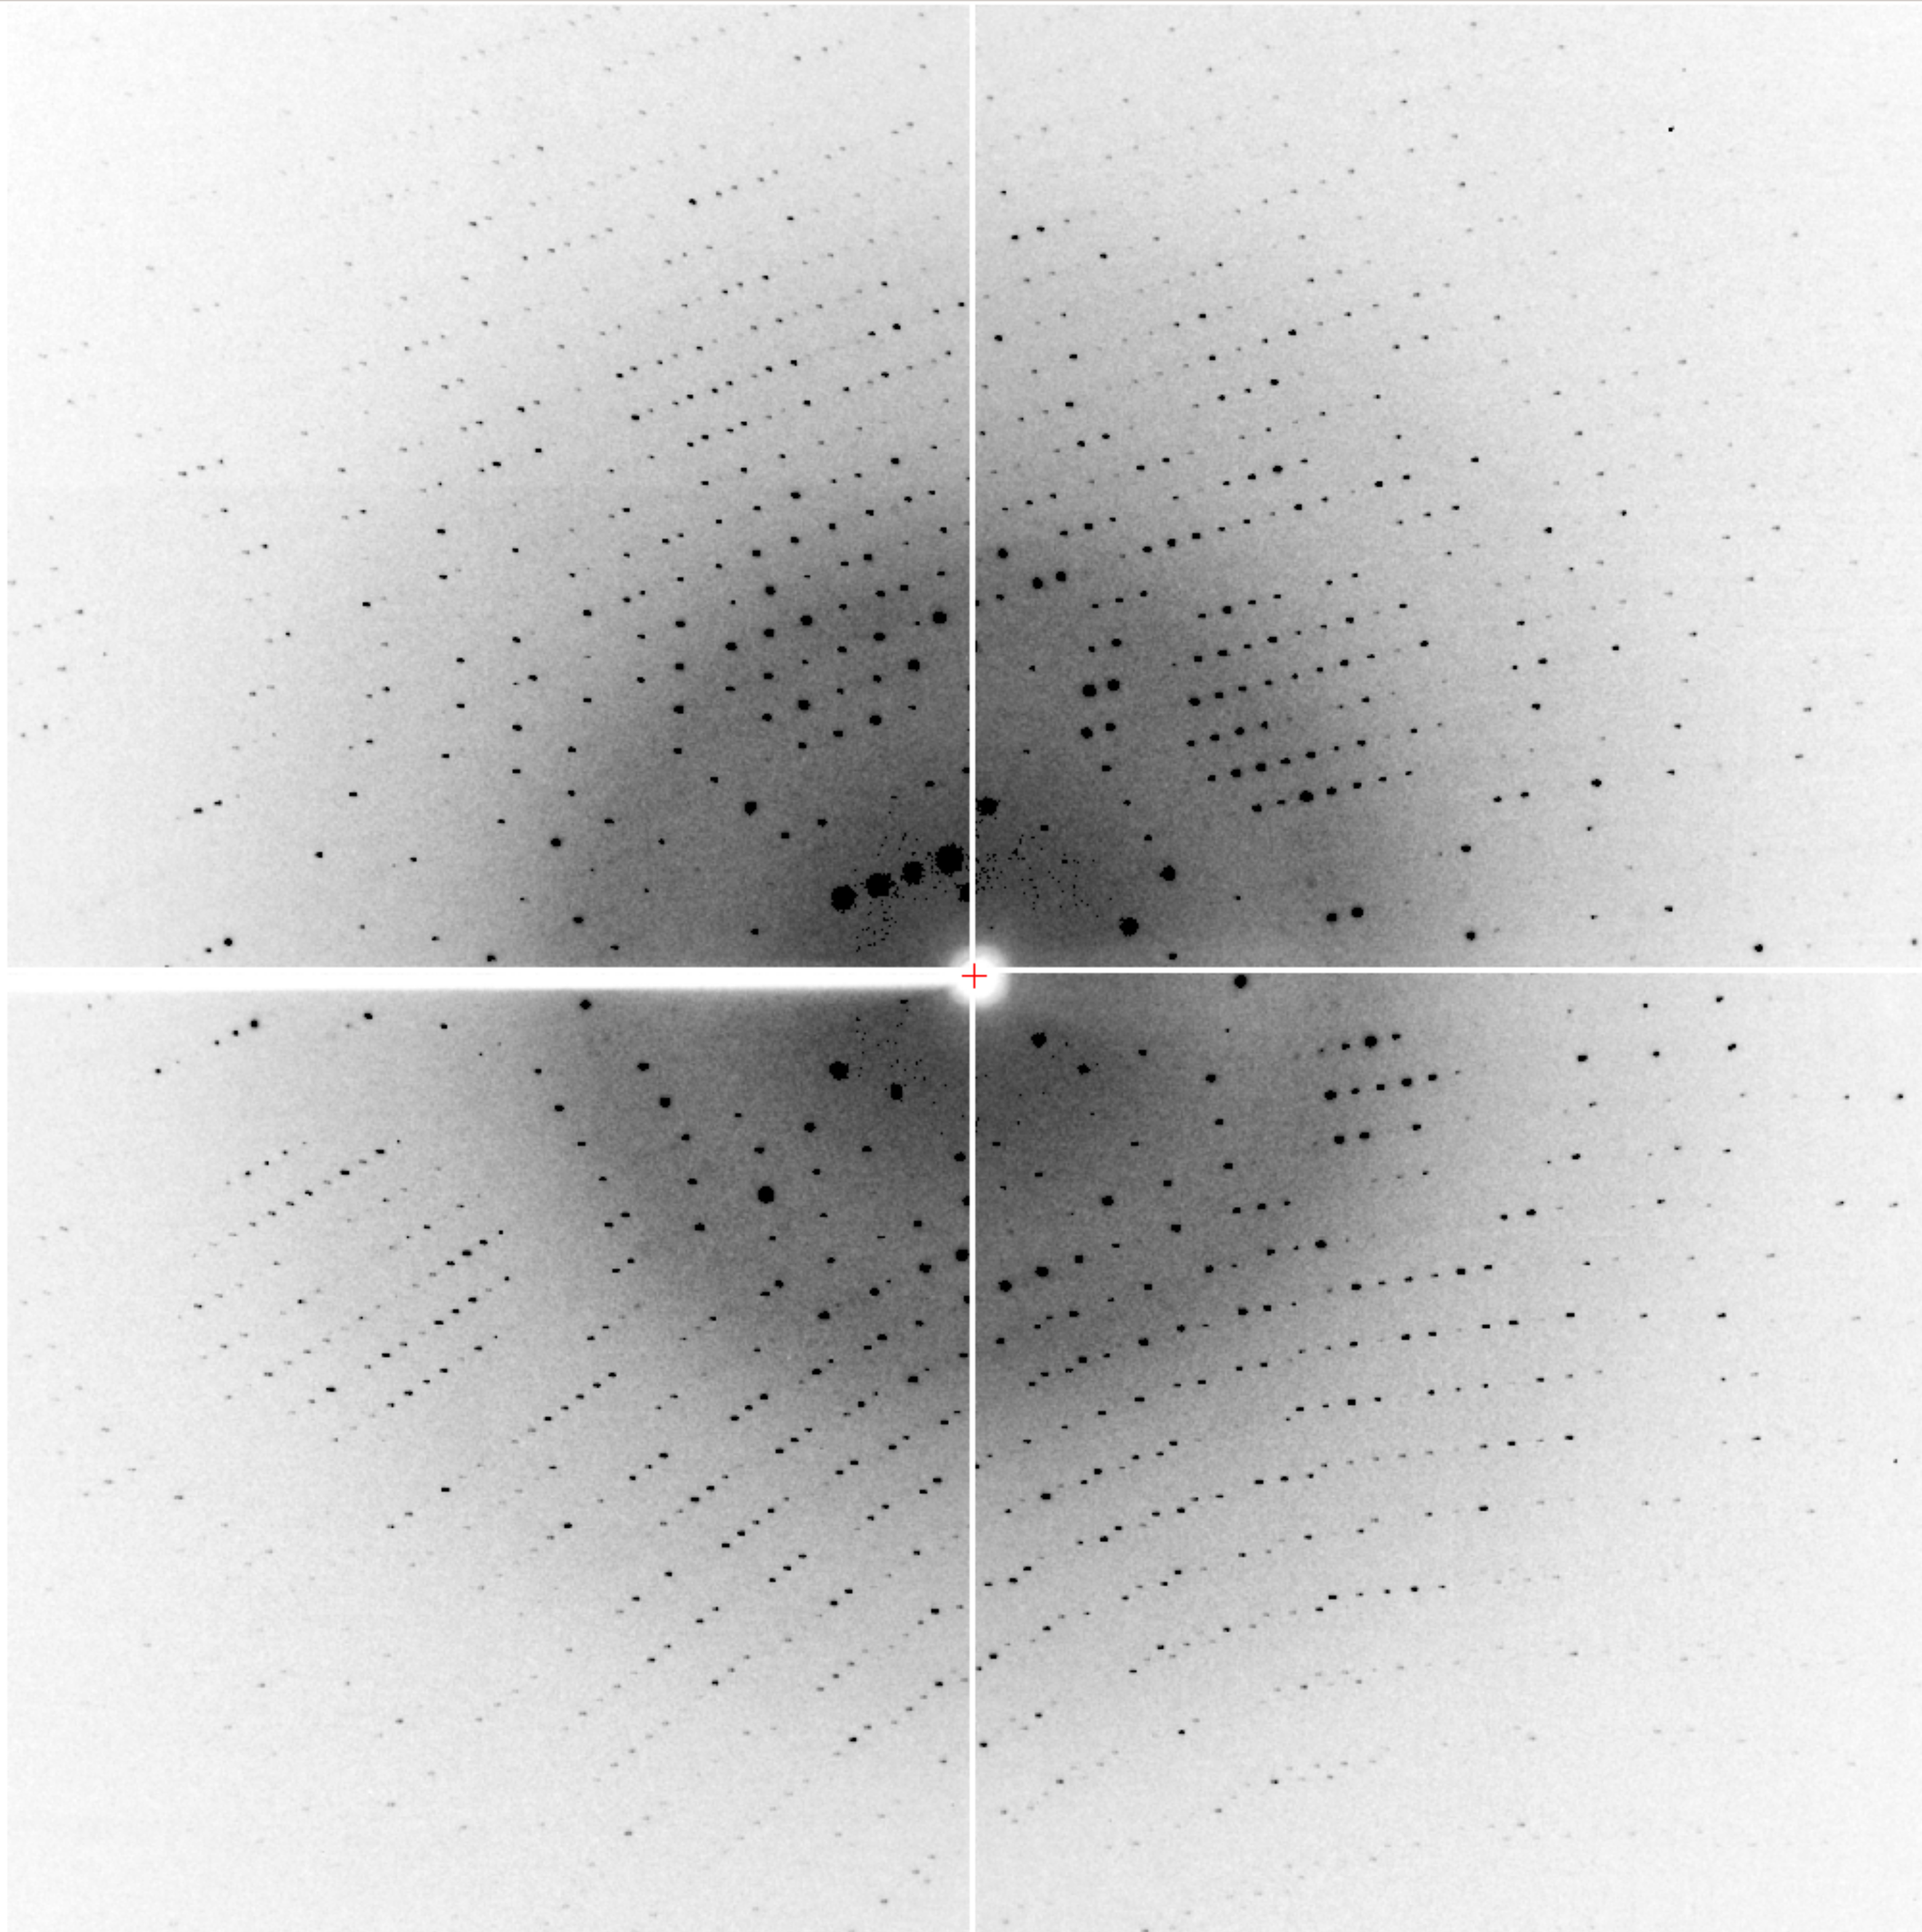
\includegraphics[width=0.9\textwidth]{imgs/patron}
	\caption[Patrón de difracción]{Patrón de difracción de la lisozima de la clara de huevo de gallina. Disponible en el siguiente enlace \url{tinyurl.com/ydfw6asv}. La resolución es la métrica principal que determina la calidad del modelo estructural de una proteína. Anillos concéntricos en el patrón de difracción, representan lo que se conoce como fajas de resolución. Las fajas de alta/baja resolución corresponden a anillos más externos/internos.}
	\labfig{fig:patron}
\end{figure}

El objetivo del experimento de la \acrshort{crx}, es obtener un \enquote{dataset} completo, es decir, suficientes patrones de difracción para los pasos subsecuentes.

\section{Daño por radiación}
\labsec{dpr}
Una de las limitantes de la \acrshort{crx}, es el daño que causan los rayos X sobre el cristal macromolecular. Esto se conoce como daño por radiación y provoca que cada cristal macromolecular presente un límite temporal, denominado tiempo de vida útil, bajo el haz de rayos X. El daño por radiación se da porque los rayos X usados tienen una energía relativamente alta\sidenote{Más información en la siguiente sección.}. En el caso de un cristal macromolecular, su estabilidad física se da por pocas interacciones no covalentes por unidad de volumen, en comparación con un cristal de sal, por ejemplo. Por esto, su desintegración no requiere de mucha energía\sidenote{Incluso su manipulación tiene que darse con extrema precaución.}. Por otro lado, es evidente que al perderse el orden cristalino, se pierde la amplificación del proceso de difracción y en consecuencia los patrones de difracción cada vez contienen menos información. En otras palabras, la calidad del cristal decae y por lo tanto la calidad de cada patrón de difracción obtenido. El daño por radiación es la principal causa de que sea difícil obtener un \enquote{dataset} completo. 

\subsection{Origen}
El daño por radiación se da porque los electrones de las moléculas que conforman el cristal, absorben la energía de los fotones incidentes. La absorción tiene su causa en uno de dos fenómenos físicos: el efecto fotoeléctrico o la dispersión inelástica. La probabilidad de que se dé el primero es un orden de magnitud mayor que el segundo. El efecto fotoeléctrico consiste en la absorción total de un fotón por un electrón. Como consecuencia el electrón es expulsado de su orbital dejando una vacante electrónica, o hueco positivo (\ce{h^+}), en la molécula que lo contenía. La energía de los electrones liberados, llamados fotoelectrones, se disipa en la trayectoria que estos hayan tomado; generando miles\sidenote{El promedio de la primera energía de ionización para los átomos presentes en una proteína es de \SI{12.05}{\electronvolt}, la energía de un fotón con una longitud de onda de \SI{1}{\angstrom} es de \SI{12398.4}{\electronvolt}.} de iones, radicales libres y eventos de excitación molecular. Los radicales son especies químicas que poseen uno o más electrones desapareados, por ende su reactividad es muy alta y su tiempo de vida es particularmente corto. Una reacción en cadena de radicales libres es inminente. Si algún radical, o cualquier especie química producto de la radiación, llegase a perturbar la red de contactos cristalinos, se pierde el orden cristalino. 

\subsection{Clasificación}
El daño por radiación se clasifica de acuerdo con su escala temporal. El daño primario es la ionización dada por el efecto fotoeléctrico. El daño secundario es la subsecuente cascada de radicales libres, dependiente del tiempo y de la temperatura. El daño terciario se define como el daño macroscópico sobre el cristal\sidenote{Fisuras o cambios en su coloración, por ejemplo.}. Esto implica que una fracción suficiente de macromoléculas dentro del cristal ha sido afectada por el daño primario y secundario \sidecite{Teng2000}.

\subsection{Consecuencias}
Las consecuencias del daño por radiación se observan en: (\emph{i}) la disminución de la intensidad de los puntos en el patrón de difracción, sobre todo aquellos en las fajas de alta resolución; (\emph{ii}) un cambio del volumen de la celda unitaria, que causa la pérdida de la isomorfía cristalina; (\emph{iii}) el aumento en los parámetros de desplazamiento atómico; y (\emph{iv}) el empeoramiento de las medidas que indican la calidad global de los datos \cite{Teng2000}. El listado anterior se conoce como daño por radiación global. Por otra parte, el daño específico se refiere al daño estructural en la macromolécula cristalizada. Esto conlleva un orden dado: primero ocurre la reducción de átomos metálicos; después se da la ruptura de puentes disulfuro; luego la descarboxilación de aspartatos y glutamatos; y finalmente se pierde el grupo tiometilo de las metioninas \sidecite{Weik2000,Ravelli2000}. No todos los residuos de aminoácido susceptibles son afectados de la misma manera. Hasta el momento, las razones de esto no han sido esclarecidas. Por este motivo, aunque existen ciertos principios básicos para determinar el daño específico, es difícil predecirlo y saber de antemano el grado en que afectará el modelo estructural obtenido. En el peor escenario, puede ser imposible obtener una estructura macromolecular debido a la inherente susceptibilidad del cristal al daño por radiación o a la pérdida de isomorfía cristalina.

\subsection{Métricas}
La mejor manera de determinar el daño por radiación en un cristal macromolecular, es estimando la dosis de radiación absorbida por el cristal. La dosis depende a su vez de la composición atómica del cristal y de algunos parámetros experimentales referentes al haz de rayos X \sidecite{Murray2004}. La dosis se mide en \si{\gray} que, según el Sistema Internacional de Unidades, es equivalente a la absorción de un Joule de energía ionizante por kilogramo de material irradiado. En experimentos de \acrshort{crx} es típico encontrar valores del orden de \si{\mega\gray} \sidecite{Garman2010}. En este aspecto, se han propuesto varias métricas para cuantificar el daño por radiación en función de la dosis absorbida; sin embargo, se ha demostrado que el uso de distintas métricas puede dar diferentes resultados \sidecite{Allan2013}. Actualmente no existe una métrica que haya sido acordada por unanimidad en el campo de la \acrshort{crx}. 

El daño por radiación específico se puede visualizar al realizar colectas de datos idénticas y tomar la diferencia entre la densidad electrónica del modelo estructural de la colecta $n$ y la colecta inicial.

\begin{figure}[hb]
	\includegraphics[width=0.75\textwidth]{imgs/before}
	\includegraphics[width=0.75\textwidth]{imgs/after}
	\includegraphics[width=0.75\textwidth]{imgs/diff}
	\caption[Diferencia de densidad electrónica]{Diferencia de densidad electrónica entre colectas de datos idénticas. Arriba: primer colecta de un cristal de lisozima (dosis absorbida \SI{0.6}{\mega\gray}). En medio: segunda colecta del mismo cristal (dosis absorbida \SI{3.2}{\mega\gray}). Los mapas $2F_{\mathrm{o}}-F_{\mathrm{c}}$ y $F_{\mathrm{o}}-F_{\mathrm{c}}$ se encuentran dibujados a \SI{1}{\sigma} y $\pm$\SI{3.5}{\sigma}, respectivamente. Abajo: La diferencia de densidad electrónica entre colectas $F_{\mathrm{o,2}}-F_{\mathrm{o,1}}$. Donde la diferencia negativa (magenta) está a \SI{-3.5}{\sigma} y la positiva (cian) a \SI{3.5}{\sigma}. Nótese como prácticamente no se observa una diferencia entre los mapas $2F_{\mathrm{o}}-F_{\mathrm{c}}$ (malla azul contra malla gris); sin embargo, sí existe una diferencia del modelo estructural inicial (el mismo en las tres imágenes) con respecto a la densidad electrónica de la segunda colecta. En otras palabras, para la segunda colecta, en una fracción de las proteínas cristalizadas este puente disulfuro se ha roto. Imagen realizada con PyMOL \cite{pymol} y datos de \cite{Nanao2005}. }
	\labfig{fig:difden}
\end{figure}


\section{Crioprotección}
\labsec{crio}
La primer estructura macromolecular determinada fue la de la mioglobina en 1958 por Kendrew y colaboradores \sidecite{Kendrew1958}. La forma de contender con el daño por radiación en aquella época era utilizando decenas de cristales y promediar los patrones de difracción. La regla de dedo para cambiar el cristal irradiado por uno nuevo, era seguir la intensidad de algunas reflexiones y si esta llegaba a disminuir de \num{20} a \SI{30}{\percent} de su valor inicial, entonces se procedía a reemplazar el cristal. 

El primer estudio en el que se valoró el potencial de la crioprotección, para reducir el daño por radiación, surgió por necesidad. Sucedía que ciertos cristales de insulina con átomos pesados sufrían un rápido desgaste por la radiación, en comparación con cristales de insulina sin átomos pesados. Con base en la observación de que el daño secundario es dependiente, en parte, de la temperatura; Low \emph{et al.} compararon, de manera cualitativa, el deterioro de los patrones de difracción colectados a \num{21}, \num{0} y a \SI{-13}{\celsius}. Los resultados fueron claros: a menor temperatura, mayor el tiempo de vida útil de los cristales  \sidecite{Low1966}. 

El problema con la reducción de temperatura en cristales macromoleculares, era la formación de hielo dentro de estos. Fue Haas quien primero usó crioprotectores para prevenir este problema. En el primer caso logró reducir la temperatura hasta \SI{-50}{\celsius}, remojando cristales de lisozima entrecruzados con glutaraldehído
en una mezcla de agua con glicerol \sidecite{Haas1968}. En un estudio posterior con cristales de lactato deshidrogenasa, el proceso de entrecruzamiento destruía los cristales. En cambio, si solo eran remojados por un par de días en una solución con sacarosa, el daño por radiación era diez veces menor \sidecite{Haas1970}. 
Es hasta 1988 que Hope describe por primera vez lo que conocemos hoy en día como criocristalografía de rayos X, donde básicamente se añade al cristal, o a la condición de cristalización, un crioprotector y el proceso de difracción del cristal se realiza a \SI{-173}{\celsius} \sidecite{Hope1988}. Una de las desventajas de esta técnica es encontrar las condiciones de crioprotección adecuadas para cada macromolécula. A pesar de este detalle, la crioprotección fue ganando adeptos de tal forma
que para el año 2000 era parte de la rutina de la \acrshort{crx} \sidecite{Garman2003}. Gracias a la crioprotección, en general era suficiente un único cristal macromolecular para obtener un
\enquote{dataset} completo.

\section{Sincrotrones}
\labsec{sincro}
La principales fuente de rayos X para realizar el experimento de \acrshort{crx}, es la radiación sincrotrón.
La historia tecnológica de los sincrotrones se divide en generaciones. La primera generación de sincrotrones eran aquellos pertenecientes al campo de la física de partículas, donde los primeros estudios con respecto a la estructura de proteínas fueron realizados \sidecite{Phillips1976}. Para la década de 1980 se construyen los sincrotrones dedicados a la biología estructural, esta es la segunda generación. Para la década de 1990 llega la tercera generación. El primer sincrotrón perteneciente a la cuarta generación empezó a operar en 2016 \sidecite{Owen2016}. 
Una de las características de un sincrotrón es su brillo espectral, que se define como la distribución del flujo de fotones en el espacio y el rango angular. El flujo se establece como el número de fotones por segundo que atraviesan un área definida por un ancho de banda dado \sidecite{Willmott2019}. La revolución tecnológica de los sincrotrones se nota en la diferencia del orden de magnitud del brillo espectral \cite{Willmott2019}. Este aumento en brillo se ha permitido pues permite una gran ventaja: la posibilidad de utilizar cristales de menor tamaño. Esto es porque la principal limitante de la \acrshort{crx} es obtener cristales macromoleculares, en particular cristales de un tamaño adecuado (al menos unos cien micrómetros en sus tres dimensiones\sidenote{Existen líneas especiales donde existe la posibilidad de usar cristales con un orden de magnitud menor, las denominadas líneas microfoco.}.) 

Actualmente se está desarrollando la tecnología para cambiar la metodología de la colecta de datos, usando cristales macromoleculares nanométricos y con una fuente de rayos X más poderosa denominada \acrshort{xfel} (del inglés \emph{X-ray Free Electron Laser}). Existen ya varios estudios en los que se ha demostrado la posibilidad de obtener estructuras macromoleculares con esta nueva metodología \sidecite{Martin-Garcia2016}. Sin embargo, el acceso al tiempo experimental en un XFEL es actualmente muy limitado.

Como se mencionó en la sección anterior, ya para el año 2000, la noción general en el campo de la criocristalografía era que el daño por radiación era insignificante, un problema del pasado. Precisamente esta noción cambia en ese mismo año, cuando tres estudios independientes muestran el efecto del daño por radiación en la entonces nueva generación de sincrotrones \sidecite{Teng2000,Weik2000,Ravelli2000}. 

\section{Radioprotectores}
\labsec{radio}
Al ser evidente que el daño por radiación aumentaba con el incremento en brillo, fue necesario buscar estrategias, como la crioprotección, que ayudaran a mitigar el daño por radiación. En el curso de los últimos veinte años, se han investigado varias estrategias pre y posteriores a la difracción con distintos enfoques \sidecite{Garman2017}. Una de las tantas estrategias, es el uso de moléculas pequeñas que interactuan con los radicales libres generados por la radiación. Estas moléculas se denominan radioprotectores. Sin embargo, en la literatura científica existen varias incongruencias con respecto a la efectividad de los radioprotectores y es por esto que la comunidad cristalográfica no ha adoptado al cien por ciento el uso de radioprotectores de manera rutinaria \sidecite{Nowak2009, Allan2013}.

%\chapter{Antecedentes}
\labch{antec}
\section{pH}
\labsec{ph}
Una estrategia innovadora, investigada en la tesis de maestría del presente autor%\sidenote{Disponible en el siguiente enlace \url{https://github.com/murpholinox/tesis\_maestria}}
, fue modificar el pH dentro de los cristales macromoleculares. Esta idea se basa en la idea general de los radioprotectores y se detalla a continuación. 

La radiólisis del agua produce las siguientes reacciones \sidecite{VonSonntag2006}:
\begin{align}
	\ce{H2O           &->[rayos X]     H2O^{.+}    +             e^{-}}  \\
	\ce{H2O           &->[rayos X]     H2O^{*}}                          \\
	\ce{H2O^{.+}      &->  \color{red}HO^{.}       +              H^{+}} \\
	\ce{e^{-} + nH2O  &->  \color{red}e^{-}_{solv.}}                     \\
	\ce{H2O^{*}       &->  \color{red}HO^{.}       +   \color{red}H^{.}}
\end{align} 
Donde las especies químicas denotadas en rojo, representan los primeros radicales libres presentes en un cristal macromolecular (el radical hidroxilo, el electrón solvatado y el radical hidrógeno).% Esto es relevante porque en general el contenido de solvente, agua, en un cristal macromolecular es bastante. 

Con la criocristalografía de rayos X, se impide la difusión del radical hidroxilo \sidecite{Owen2012a}. Sin embargo, el \ce{e^{-}_{solv.}} y el radical hidrógeno todavía son móviles. El electrón solvatado puede moverse del solvente a la proteína, donde es capaz de viajar a través de la cadena polipeptídica hasta hallar un centro electrofílico, como por ejemplo átomos metálicos o puentes disulfuro (véase la \reffig{fig:symons92}) \sidecite{Symons1997}. Esta es la razón del origen del orden en el que se presenta el daño por radiación específico, pues la captura de electrones es mucho más específica que la captura de huecos positivos \sidecite{Close2019}. Por su parte, el radical hidrógeno sigue una reacción de recombinación formando como producto final \ce{H2}, al parecer el responsable directo del daño por radiación global \sidecite{Meents2010}.

\begin{figure}[h]
	\centering
	\includegraphics[width=0.9\textwidth]{imgs/symons92.png}
	\caption[Movimiento de cargas en la cadena polipeptídica]{Moviento de electrones (a) y huecos positivos (b), a través de la cadena polipeptídica. Fuente: \cite{Symons1997}.}
	\labfig{fig:symons92}
\end{figure}

El electrón solvatado y el átomo de hidrógeno se encuentran en un equilibrio ácido-base; por lo que el electrón solvatado se convierte en \ce{H^{.}} en una solución ácida. %De hecho, en el campo de la química de las radiaciones, es común estudiar el efecto de un radical al convertir los otros radicales en especies el radical estudiado. 
\begin{equation}
\ce{e^{-}_{solv.} + H^{+} <=> H^{.}}
\end{equation}

En la tesis de maestría se usó como sistema de estudio la lisozima de clara de huevo de gallina, que presenta cuatro puentes disulfuro. La idea era que el ion hidronio, también conocido como oxidanio, funcionara como radioprotector al interactuar con los electrones solvatados antes que estos interactuaran con los puentes disulfuro de esta proteína. Para esto, se comparó el daño específico sobre los puentes disulfuro en cristales de lisozima a tres niveles de p: \num{3.7}, \num{4.7} y \num{5.7}. Los resultados obtenidos fueron opuestos a los esperados: a niveles comparables de dosis de radiación absorbida, el cristal con el pH más ácido presentó mayor daño por radiación que el cristal con el pH más básico.

La variabilidad entre cristales macromoleculares, aún proveniendo de la misma condición de cristalización, puede llevar a conclusiones erróneas \sidecite{Nowak2009}. En la tesis de maestría no se pudo concluir si la diferencia observada era estadísticamente significativa, pues no se realizaron las repeticiones necesarias para cada condición experimental.



%\input{chaps/objet}
%\input{chaps/mayme}

%\pagelayout{wide} % No margins
%\addpart{Class Options, Commands and Environments}
%\pagelayout{margin} % Restore margins

\appendix % From here onwards, chapters are numbered with letters, as is the appendix convention

%\input{chaps/apend}
%\input{chaps/apend2}

%----------------------------------------------------------------------------------------

\backmatter % Denotes the end of the main document content
\setchapterstyle{plain} % Output plain chapters from this point onwards

%----------------------------------------------------------------------------------------
%	BIBLIOGRAPHY
%----------------------------------------------------------------------------------------

% The bibliography needs to be compiled with biber using your LaTeX editor, or on the command line with 'biber main' from the template directory

\defbibnote{bibnote}{Here are the references in citation order.\par\bigskip} % Prepend this text to the bibliography
\printbibliography[heading=bibintoc, title=Bibliografía, prenote=bibnote] % Add the bibliography heading to the ToC, set the title of the bibliography and output the bibliography note

%----------------------------------------------------------------------------------------
%	NOMENCLATURE
%----------------------------------------------------------------------------------------

% The nomenclature needs to be compiled on the command line with 'makeindex main.nlo -s nomencl.ist -o main.nls' from the template directory

%\nomenclature{$c$}{Speed of light in a vacuum inertial frame}
%\nomenclature{$h$}{Planck constant}

%\renewcommand{\nomname}{Notation} % Rename the default 'Nomenclature'
%\renewcommand{\nompreamble}{The next list describes several symbols that will be later used within the body of the document.} % Prepend this text to the nomenclature

%\printnomenclature % Output the nomenclature

%----------------------------------------------------------------------------------------
%	GLOSSARY
%----------------------------------------------------------------------------------------

% The glossary needs to be compiled on the command line with 'makeglossaries main' from the template directory

%\setglossarystyle{listgroup} % Set the style of the glossary (see https://en.wikibooks.org/wiki/LaTeX/Glossary for a reference)
%\printglossary[title=Special Terms, toctitle=List of Terms] % Output the glossary, 'title' is the chapter heading for the glossary, toctitle is the table of contents heading

%----------------------------------------------------------------------------------------
%	INDEX
%----------------------------------------------------------------------------------------

% The index needs to be compiled on the command line with 'makeindex main' from the template directory

\printindex % Output the index

%----------------------------------------------------------------------------------------
%	BACK COVER
%----------------------------------------------------------------------------------------

% If you have a PDF/image file that you want to use as a back cover, uncomment the following lines

%\clearpage
%\thispagestyle{empty}
%\null%
%\clearpage
%\includepdf{cover-back.pdf}

%----------------------------------------------------------------------------------------

\end{document}
